
\chapter{Ergebnisse}

\section{Bildqualität}
Leider ist es uns hardwarebedingt nicht m\"oglich aussagekr\"aftige Bilder 
gegen\"uberzustellen. Durch Verringer der Kamerafrequenz wird die Bildqualit\"at bereits erheblich reduziert. 

\begin{figure}[htpb]
\begin{center}
\subfigure[RAW]{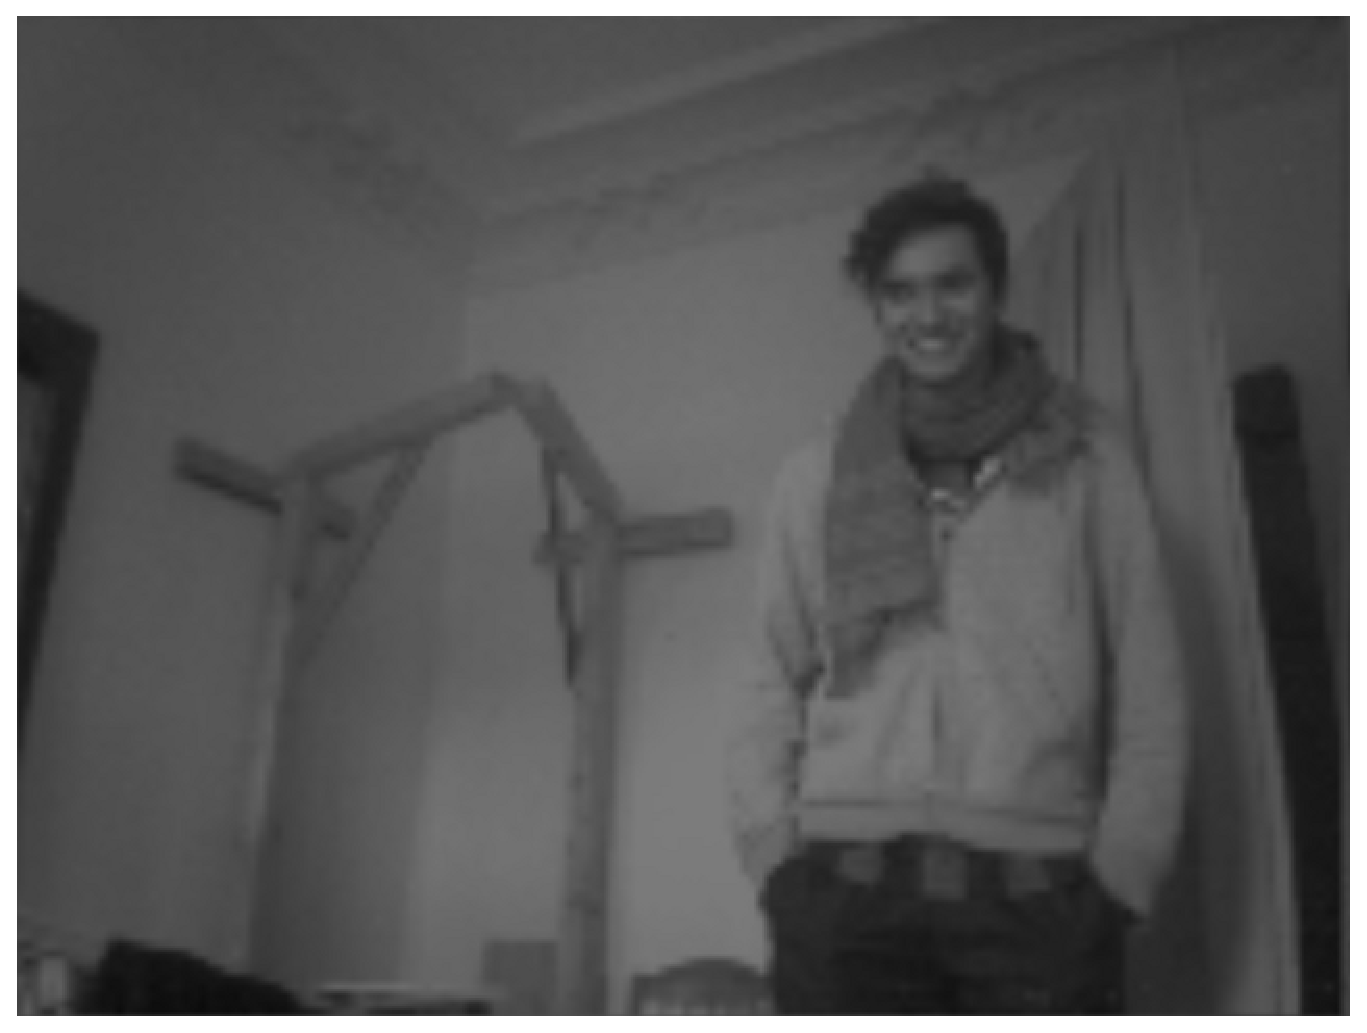
\includegraphics[width=0.3\textwidth]{img/sample-raw}}
\subfigure[2D]{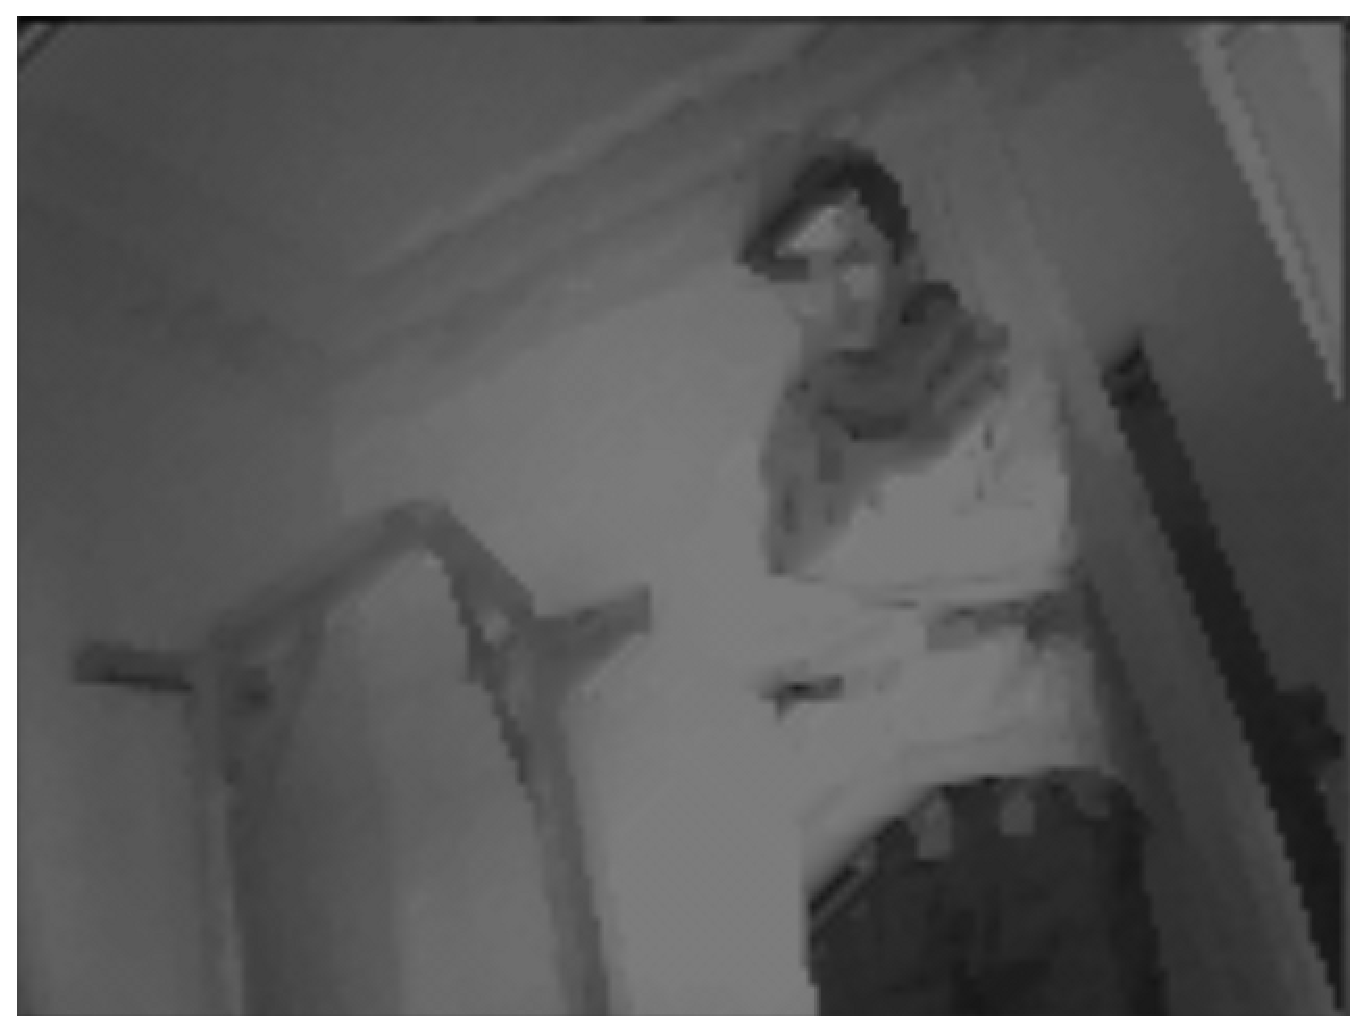
\includegraphics[width=0.3\textwidth]{img/sample-cmpr}}
\subfigure[3D]{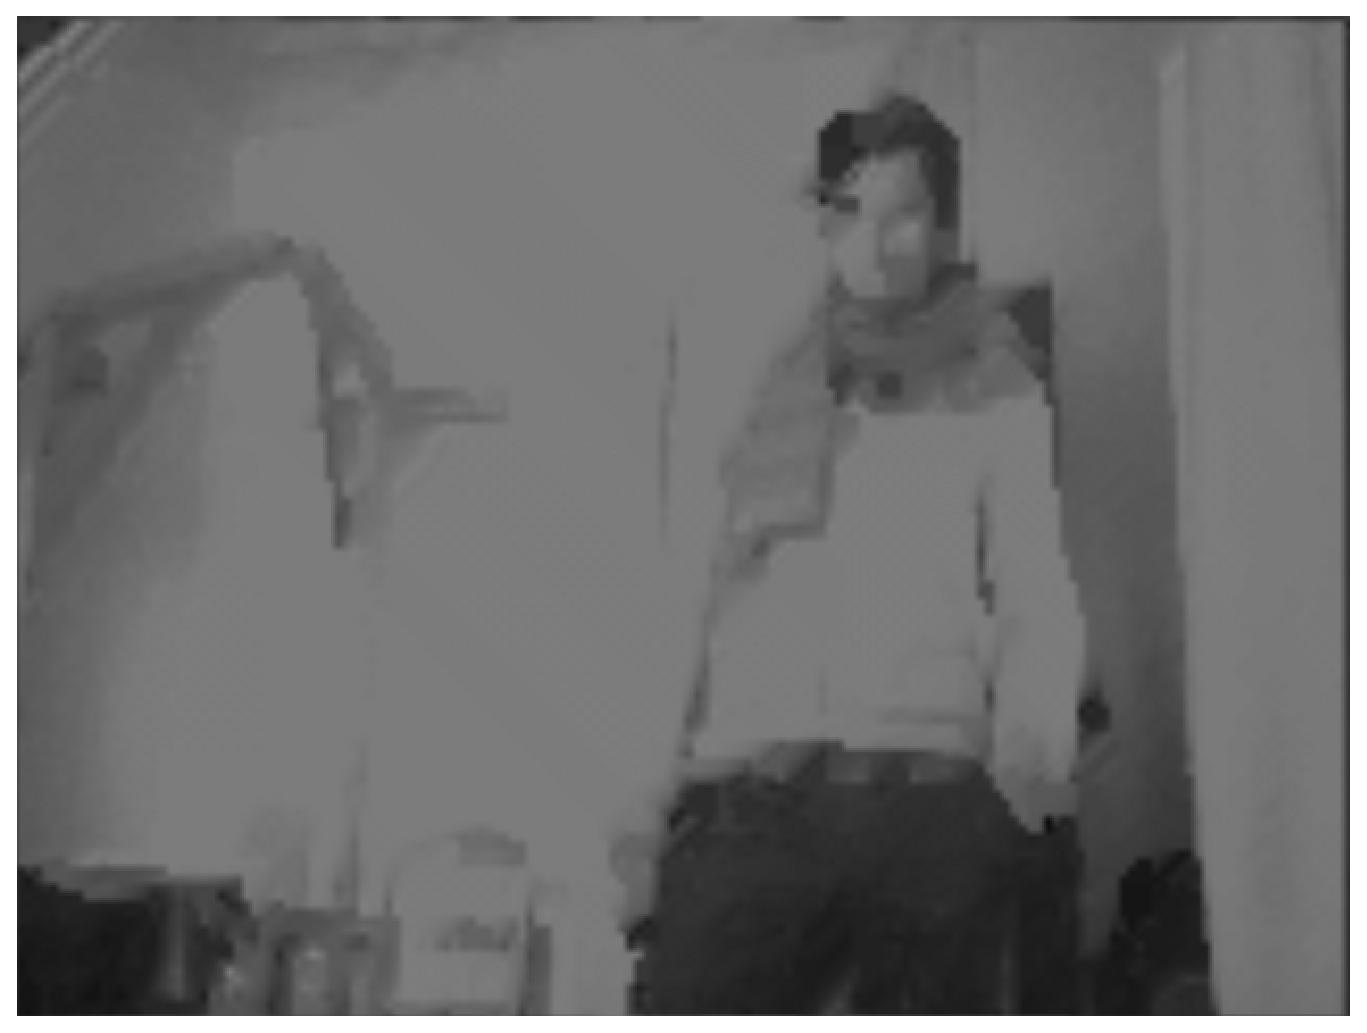
\includegraphics[width=0.3\textwidth]{img/sample-cmpr3}}
\end{center}
\caption{RGB - Bayer - RGB Transformation auf 16x16 Pixel Bild}
\label{fig:sample}
\end{figure}

Sowohl bei 2D wie auch bei 3D Komprimierung sind die Artefakte sichtbar,
die sich auf dem Bild befindende Objekte sind aber gut erkennbar:


\section{Komprimierung}
\begin{table}[hp]
\centering
\begin{tabular}{|l|r|}
\hline
      x     & bytes/frame   \\
\hline
raw         & 19200         \\
cmpr        &  5040         \\
cmpr3 (rle) & $\approx$3200 \\
\hline
\end{tabular}
\caption{Gegen\"uberstellung der Komprimierung}
\end{table}


\section{Performance}

\begin{table}
\centering
\begin{tabular}{|l|l|l|l|}
\hline
      & \multicolumn{2}{|c|}{Framerate mit Test-Video}     & \multicolumn{1}{|c|}{Frequenz mit Camera}      \\
      & mit En- und Decodierung & Encodierung und Netzwerk & Encodierung und Netzwerk \\
\hline
raw   & 133 &  52 & 6/10 \\
cmpr  &  48 &  54 & 12/5 \\
cmpr3 &  26 &  27 & 28/2 \\
\hline
\end{tabular}

\caption{Performance der Codecs}
\end{table}

